\chapter{Contexto}

\subsection{Cadena 'no es mayor que'}

\newpage
\subsection{Esquema general}
	\begin{figure}[h!]
		%width=\textwidth
		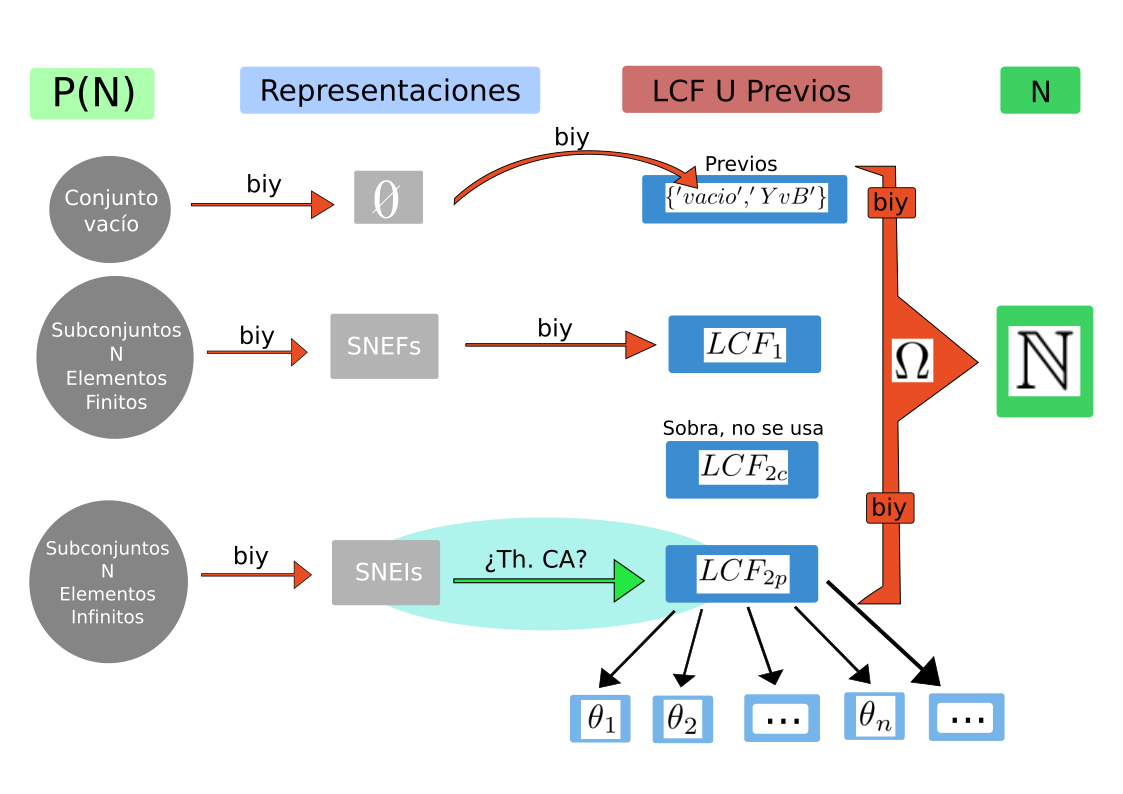
\includegraphics[ scale=0.7, angle=90]{EsquemaRelaciones}
		%\includegraphics[width=\textwidth, scale=0.3]{Funcion_hx_002_v4}
		%\includegraphics[width=\textwidth, scale=0.3]{Funcion_hx_001_v4}
		\centering
	\end{figure}

\newpage
\subsection{Definiciones}
\subsubsection{Cadenas de subconjuntos y particiones}
\subsubsection{SNEF}
\subsubsection{SNEI}
\subsubsection{LCF U previos}



\newpage
\subsection{Sentido cardinal de las soluciones multiverso}